\documentclass[a4paper,12pt]{article}
\usepackage[utf8]{inputenc}
\usepackage[english]{babel}
\usepackage[utf8]{inputenc}
\usepackage{graphicx, array, blindtext}
\usepackage[colorinlistoftodos]{todonotes}

\DeclareUnicodeCharacter{2212}{-}

\usepackage [a4 paper , hmargin =1.2 in , bottom =1.5 in] {geometry}
\usepackage [parfill] {parskip}

\usepackage{enumitem}
\usepackage{amsmath}
\usepackage{amsthm}
\usepackage{amssymb}
\usepackage [linesnumbered, ruled, vlined] {algorithm2e}
\usepackage{listings}
\usepackage{xcolor}
\usepackage{floatrow}
\bibliographystyle{plainurl}
\bibliography{biblio}
\usepackage{amssymb}   
\usepackage{hyperref}
\usepackage{cancel}
\usepackage{fancyhdr}
\usepackage{graphicx}
\usepackage{verbatim}
\usepackage{dirtytalk}
\usepackage[document]{ragged2e}
\newcommand{\comment}[1]{}
\hypersetup{pdftitle={main.pdf},
    colorlinks=false,
    linkbordercolor=red
}

\newtheorem{definition}{Definition}
\numberwithin{definition}{section}
\newtheorem{mytheorem}{Theorem}
\numberwithin{mytheorem}{subsection}

\newcommand{\latex}{\LaTeX\xspace}
\newcommand{\tex}{\TeX\xspace}    
\urlstyle{same}
\pagestyle{fancy}
\fancyhf{}
\rhead{Software Systems Laboratory}
\lhead{200050013-200050130}
\fancyfoot[C]{Page \thepage}



%opening

\centering{

\title{\fontsize{150}{60}{Outlab 2: \latex and gdb}}\\ 




\author{

Arpon Basu  \\
        Shashwat Garg }

}





\date{Autumn 2021}
\begin{document}
\renewcommand{\refReferences}{} % this is for changing the heading of bibliography
\maketitle


\tableofcontents

\newpage
\justifying
\section{Basic Theory of Linear Recurrences}
We all know about the Fibonacci Sequence, given by the recurrence\\


\makebox[\linewidth]{$f_{n+2} = f_{n+1} + f_{n}$}

\\
and initialised as $f_0 = 0,$ $f_1 = 1$. This is an instance of what is called a Linear Recurrence Sequence, or LRS.\\
\begin{definition}
LRS $(u_n)^\infty_{n=0}$ of order $k$ over field $\mathbb{F}$ is the sequence determined by the recurrence\\
\begin{equation}
\makebox[0]{$u_{n+k} = \sum\limits_{j=0}^{k-1} a_{j}u_{n+j}$}
\end{equation}\\
for integers $n$ $\geq$ \emph{0} with $a_0 , . . . , a_{k−1} \in \mathbb{F}, a_0 \neq 0$, and an initialisation vector\\
\makebox[\linewidth]{$\begin{bmatrix} $u_0$ & ... & $u_{k-1}$ \end{bmatrix}^{T} \in \mathbb{F}^{k \times 1}$}

\end{definition}\\
Thanks to Definition 1.1, when we say that we are given $(u_n)^\infty_{n=0}$
 of order $k$ over $\mathbb{F}$, we actually mean that we are given the 2$k$ constants $a_0 , . . . a_{k−1} , u_0 , . . . , u_{k−1} \in \mathbb{F}$.\\
The Fibonacci sequence shows up a lot in pop culture and DSA assignments, however, the study of LRS is a vast subject in its own right, with applications in software verification, quantum computing, formal languages, statistical physics, combinatorics, and theoretical biology, to name a few.
\subsection{Computing terms of an LRS}
For a fixed $k$, assuming we can do arithmetic operations in $\mathbb{F}$ in constant time, how long does it
take to compute the $n^{th}$ term of a given LRS?\\
\begin{algorithm}[ht]
\caption{Naive first attempt \textsf{naive}}
\SetAlgoLined
\DontPrintSemicolon
\KwData {LRS $(u_n)^\infty_{n=0}$, $n$}
\KwResult {$u_n$}
\uIf {$n < k$}  
{\textbf{return} $u_n$}\\
\textbf{end}\\
\textbf{return} $\sum_{j=0}^{k-1} a_{j}\cdot$\textsf{naive}$((u_n)^\infty_{n=0}, n - k + j)$ 
\end{algorithm}\\
By the way, notice the use of $\textsf{\textbackslash mathsf}$ to write \textsf {“naive”} . This algorithm, unfortunately, is painfully
inefficient: as you can see, the number of recursive calls will be exponentially many in $n$. This
immediately prompts a more “bottom-up” 3 approach: we start from the first k terms, use them
to compute the next term, and iterate this way upto n. This takes $\mathcal{O}(n)$ iterations.\\
But we can do better, in fact, we only need $\mathcal{O}$(log $n$) iterations. 4\\
Technically, even Algorithm 2 is \emph{inefficient}: when we analyse complexity, we do it with respect to
the size of the \emph{bit representation} of the input, i.e. how many bits it takes to specify the input. An
integer $n$ takes log $n$ bits to represent, so the parameter for describing complexity is not $n$, but
$\eta$ = log $n$.\\
\begin{algorithm}[ht]
\caption{Bottom up dynamic programming approach  \textsf{bottomup}}
\SetAlgoLined
\DontPrintSemicolon
\KwData {LRS $(u_n)^\infty_{n=0}$, $n$}
\KwResult {$u_n$}
\uIf {$n < k$}  
{\textbf{return} $u_n$}\\
\textbf{end}\\
\textsf{circularArray} $\longleftarrow$ \{$u_0$ , . . . $u_{k−1}$\}\\
\textsf{arrayStartIndex} $\longleftarrow$ 0\\
$n_{last}\longleftarrow k - 1$\\
\While {$n_{last} < n$}{
\textsf{nextTerm}\longleftarrow$\sum_{j=0}^{k-1} a_{j}\cdot$\textsf{circularArray[(arrayStartIndex} + $j\textsf{)}\%k\textsf{]}$\\
\textsf{arrayStartIndex} $\longleftarrow$ (\textsf{arrayStartIndex} + 1)\%$k$\\
$n_{last}\longleftarrow n_{last} + 1$
}\\
\textbf{return} \textsf{circularArray[(arrayStartIndex} + $k - 1$\textsf{)}\%$k$\textsf{]}
\end{algorithm}
\\
Yes, we can compute the $n^{th}$ term with $\mathcal{O}(\eta)$ operations, and the trick here is a method called \textbf{iterated squaring}. Given an LRS $(u_n)^\infty_{n=0}$, define its companion matrix \textbf{M} $\in \mathbb{F}^{k \times k}$ as\\
\begin{equation}
\makebox[0]{
\textbf{M} = 
  
 \begin{bmatrix} 
    0 & 1 & 0 & \dots & 0 \\
    0 & 0 & 1 & \dots & 0 \\
    \vdots & \vdots & \vdots & \ddots & \vdots \\
    0 & 0 & 0 & \dots & 1\\
    a_0 & a_1 & a_2 & \dots & a_{k-1}\\
    \end{bmatrix}



}
\end{equation}\\
Compare equations 1 and 2 and observe that\\
\begin{equation}
\makebox[0]{
\textbf{M}^{n}
  
 \begin{bmatrix} 
    u_0 \\
    \vdots  \\
    u_{k-1}\\
    
    \end{bmatrix}
 = 
 \begin{bmatrix} 
    u_n \\
    \vdots  \\
    u_{n+k-1}\\
    
    \end{bmatrix}


}
\end{equation}\\



Iterated squaring hinges on this ridiculously trivial observation: consider the (unique!) binary
representation of $n$: if you append a 0 to it, it becomes 2$n$, if you append a 1, it becomes 2$n$ + 1.\\
Given \textbf{M}, to compute \textbf{M}$^{n}$ , all we have to do is start with \textbf{I}, read the binary representation of $n$ from
most to least significant: if at some point we have \textbf{M}$^{j}$ , \textbf{M}$^{j}$ $\cdot$ \textbf{M}$^{j}$ = \textbf{M}$^{2j}$ , \textbf{M}$^{2j}$ · \textbf{M} = \textbf{M}$^{2j+1}$.\\

In Algorithm 3, we use a data structure called a \textbf{stack}. The constant time operations it supports
are
\begin{itemize}
\item pushing an element onto the top of the stack
\item popping an element from the top of the stack (i.e. deleting the topmost element)
\item reading the topmost element
\item checking whether the stack is empty
\end{itemize}
As you can see, it’s Last In, First Out.\\
The division while loop gets the bits of $n$ from least to most significant, the iterated square while
loop uses the bits from most to least significant. A stack fits the bill.\\
\begin{algorithm}[ht]
\caption{Iterated squaring approach \textsf{efficient}}
\SetAlgoLined
\DontPrintSemicolon
\KwData {LRS $(u_n)^\infty_{n=0}$, $n$}
\KwResult {$u_n$}
\textsf{quotient}\longleftarrow n\\
\textsf{operationStack}\longleftarrow \{\}\\
\textbf{M}\longleftarrow \textsf{companion}((u_n)^\infty_{n=0})\\
\textbf{x}\longleftarrow \begin{bmatrix} u_0 & ... & u_{k-1} \end{bmatrix}^{T}\\
\textbf{A}$\longleftarrow$$\textbf{I}_{k\times k}$\\
\While {\textsf{\emph{quotient}} $\neq$  \emph{0}}  
{\textsf{push(operationStack, quotient\%2)\\
quotient $\longleftarrow$ quotient/2}}\\
\While {\textsf{\emph{operationStack}} $\neq$ \{\}   }  
{
\textbf{A}\longleftarrow\textbf{A}\cdot\textbf{A}\\
\uIf {\emph{\textsf{top(operationStack)} = 1}}  
{\textbf{A}\longleftarrow\textbf{A}\cdot\textbf{M}}\\
\EndIf
\textsf{pop(operationStack)}}

\\
\textbf{y}\longleftarrow\textbf{Ax}\\
\textbf{return y}[0] 
\end{algorithm}
\\

\subsection{Problems associated with LRS}

Surprisingly, the following rather simple decision problem 5 , referred to as the Skolem problem,
has been open for the last eight decades or so.\\

\begin{definition}
\emph{(Skolem problem)}. For the arbitrary LRS $(u_n)^\infty_{n=0}$ whose description is given as
input, does there exist an integer $n \geq 0$ such that $u_n = 0$?
\end{definition}
This has a bunch of equivalent formulations, and by being open, we mean that nobody really knows of an algorithm that can decide it (the algorithm should terminate and give the correct
answer for \emph{all} possible inputs), or whether there is such an algorithm at all.\\
We can also consider another related problem for LRS over fields where the $>$ operator is defined:\\
\begin{definition}
\emph{(Positivity problem)}. For the arbitrary LRS $(u_n)^\infty_{n=0}$ whose description is given as
input, is it the case that for all integers $n \geq 0$, $u_n \geq 0$?
\end{definition}
Deciding even special cases of these problems (i.e. restricting what kind of LRS can be fed as
input) requires sophisticated maths, like Kronecker’s theorem on Diophantine approximations, [2,
Chap. 7, Sec. 1.3, Prop. 7], and profound properties of “algebraic” numbers [3] and then some
more mathematical arsenal [1, 4].\\
If you found this short write up interesting, here is a survey talk about the problem, given not so
long ago.
\newpage
\section{Programming}
In this section, we describe what we observe while running code (read the comments before
int main for how to use) that tries to implement Algorithm 3 of Section 3.1. So we go\\
\texttt{\# g++ iterate\_buggy.cpp -o executable}\\
and then\\
\texttt{\# ./executable <n> <k>}\\
and boom, there’s a segfault (i.e. the program is trying to access a memory address that isn’t
allocated to it). We don’t really need to go scanning through the code, inserting print statements.
We’re going to use gdb. So we go,\\
\texttt{\# g++ -g iterate\_buggy.cpp -o executable}\\
and then\\
\texttt{\# gdb -tui --args executable <n> <k>}.\\
Hit enter till the code shows up on the interface. At this point, take a screenshot.\\
Now, enter\\
\texttt{(gdb) r}\\
in the prompt, and the program runs, and segfaults. You can track the offending line exactly with\\
\texttt{(gdb) bt}\\
which is short for backtrace, and in this context, has nothing to do with online semesters. This
command prints out the program stack, and you can see the sequence of function calls that led to
this point. Take another screenshot of this output. In this example, the mistake is pretty trivial,
and you can fix it.\\
You now have two screenshots, put them in your PDF side by side, like this: (we will put two
unrelated images in the original as placeholders)\\
\begin{minipage}{0.3\textwidth}
      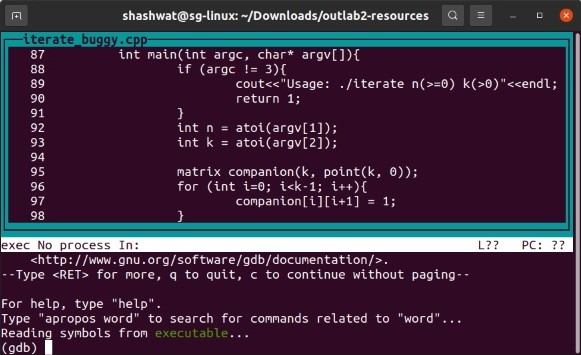
\includegraphics[width=1.5\linewidth, keepaspectratio]{First Screenshot.jpeg}
    \end{minipage}
\begin{minipage}{0.3\textwidth}
    \hbox{\hspace{-1.5em}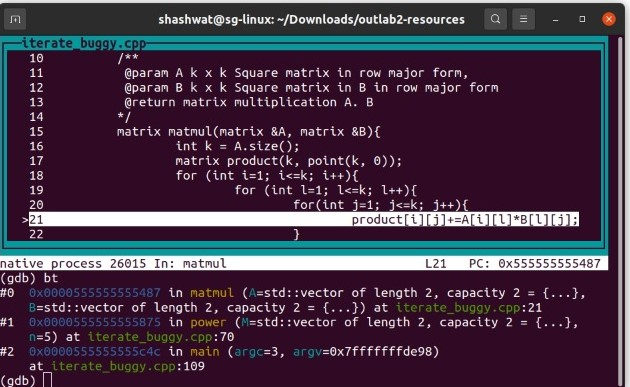
\includegraphics[width=1.5\linewidth, keepaspectratio]{Second Screenshot.jpeg}}  
    \end{minipage} \\   
For correctness, you can conveniently check with Fibonacci, as the answers are easily available
online. It turns out, that after your small fix, the code exits normally, but gives the wrong
answers.\\
What you can do is navigate the program, line by line. Set breakpoints where you want to pause,
it can be a line number, or the name of a function, like\\
\texttt{(gdb) b 42}\\
or\\
\texttt{(gdb) b main}\\
If you have paused, and want to fast forward upto some line, say 42, you can issue\\
\texttt{(gdb) until 42}\\
Or if you want to continue till the next breakpoint, simply\\
\texttt{(gdb) c}\\
To execute the next line, without stepping into the functions, you go\\
\texttt{(gdb) n}\\
If you want to step into the function call present in the next line, you go\\
\texttt{(gdb) s}\\
instead. You can print pretty much any expression (even entire vectors or STL containers) with\\
\texttt{(gdb) print <expression>}\\
Instead of breakpoints, you can set watchpoints with variables: pause whenever a variable is modified\\
\texttt{(gdb) watch <variable>}\\
You can remove breakpoints and watchpoints:\\
\texttt{(gdb) info breakpoints}\\
\texttt{(gdb) info watchpoints}\\
Note the number in the Num column, and then issue\\
\texttt{(gdb) delete <number>}\\
Armed with this knowledge, and whatever else you learn from \texttt{man gdb}, can you find out why the code gives wrong answers?\\
Once you’re sure you’ve fixed everything, consider the last three digits of your roll numbers. Add
the numbers ($<$ 1000) they form. Let this sum be $m$. Consider the smallest multiple of $m$ that exceeds 300. Let this be $n$. Use the code to compute the $n^{th}$ Fibonacci term, set a breakpoint on line 68, and complete the following:\\
\texttt{(gdb) print working}\\
\texttt{copy paste verbatim the exact output gdb gives}\\
\texttt{(gdb) print operations}\\
\texttt{copy paste verbatim the exact output gdb gives}\\
Make this table (one significant digit is ok), we will partially make it for 719.\\
\begin{center}
\begin{tabular}{ | c | c |  }
  \hline
  symbol & value  \\ \hline
  $z Na$ & 11  \\ \hline
  $z F$ & 9  \\ \hline
  $Emax Na$ & 0.545 & $[MeV]$ \\ \hline
\end{tabular}
\end{center}
\textbf{For this section, you only have to put the two screenshots, the two gdb outputs asked for, and the table in your PDF}.
\newpage
\section{Hints and tips}
Typesetting the algorithms can appear daunting, and is not covered in the tutorial, so we’ve given
you boilerplate code for that. Note that this also helps you along with some symbols, indicates
the usage of $\textsf{\textbackslash mathsf}$, and encourages the use of macros.\\
To earn bonus credit, your PDF should include this listing, and a reference to it, like so: Listing
1. The lesson on Advanced Formatting in the tutorial may help you go about defining such a
custom environment and a counter with the help of $\texttt{\textbackslash lstnewenvironment}$.\\
Also, don’t worry if you can’t place the algorithms exactly where they are with respect to the text
in the original. The entire section tells a story, and if you place the algorithms intuitively, you’ll
get more or less the same result, and that’s perfectly fine by us.\\
Just make sure to start every section on a new page.\\
Bell and Gerhold, and Renegar wrote journal articles, your bibliography entry should have the
author, title, journal, volume and year (page numbers optional).\\
Bourbaki wrote a book, the fields in your entry will be author, year, title and publisher.\\
Mignotte wrote a conference article, include author, year, title, booktitle.\\
The source project has the following files:\\
\begin{itemize}
    \item aristotle.png
    \item biblio.bib
    \item kripke.png
    \item main.tex
    \item typeset.sh
\end{itemize}

The original typeset.sh (you can create your own but don’t suppress output)
\clearpage






\pagebreak





\pagebreak


\newpage



\end{document}


